\section{2D Transonic Flow Over an Open Cavity}\label{sec:cavity}

The first case we examine is two-dimensional transonic flow over an open cavity. Flow over open cavities has been studied extensively due to its practical applications in aviation (e.g., bomb or landing gear bays) and the interesting acoustic phenomena it exhibits, particularly the resonant coupling of the cavity leading edge shear layer and acoustic feedback from the cavity trailing edge. Pioneering experimental work in the mid-1900's such as that by Roshko~\cite{Roshko1952}, Krishnamurty~\cite{Krishnamurty1955}, and Rossiter~\cite{Rossiter1964}, numerical modeling work such as that by Colonius \textit{et al.}~\cite{Colonius1999}, Rowley \textit{et al.}~\cite{Rowley2002}, and Larchev\^{e}que \textit{et al.}~\cite{Larcheveque2007}, and more recent experimental efforts such as those by Wagner\textit{et al.}~\cite{Wagner2015} and Casper \textit{et al.}~\cite{Casper2018} have investigated the effects of cavity dimensions, freestream flow regime, and turbulence on the behavior of this aeroacoustic coupling. In this work, we follow the research conducted by Tezaur et al.~\cite{Tezaur2016,Tezaur2017} in investigating PROM performance in modeling two-dimensional flow over a rectangular cavity at a Mach number of 0.6.

\subsection{Full-order Model}

The computational domain is modeled as a rectangular cavity set in a flat wall, with the leftmost, rightmost, and topmost boundaries of the domain open to the atmosphere. The geometry is shown in Fig.~\ref{fig:cavityGeom}. The cavity is $L =$ 91.71 mm long, and $D =$ 45.855 mm deep ($L/D = 2.0$). The wall extends 290.8 mm (a little over three cavity lengths) both upstream and downstream of the leading and trailing edges of the cavity, respectively, for a total domain length of 673.31 mm. The upper boundary (open to air) is set 290.8 mm from the main wall. No-slip wall boundary conditions are enforced at all walls. A characteristic inlet boundary condition is enforced at the left-most domain boundary, and characteristic outlet boundary conditions are enforced at the topmost and rightmost domain boundaries. These characteristic boundaries allow acoustic waves to exit the domain with minimal reflection. The mesh is composed of 125,000 quadrilateral cells, resulting in a total number of degrees of freedom of $\numDOF =$ 500,000. A red dot in Fig.~\ref{fig:cavityGeom} marks the location of a point monitor which will be measured throughout this section. It is placed halfway up the aft wall of the cavity, at $(x, \; y) = (91.71, \; -22.93)$ mm.

\begin{figure}
    \centering
	\ifdefined\DRAFT
		\includegraphics[width=0.9\linewidth]{example-image-a}
	\else
    	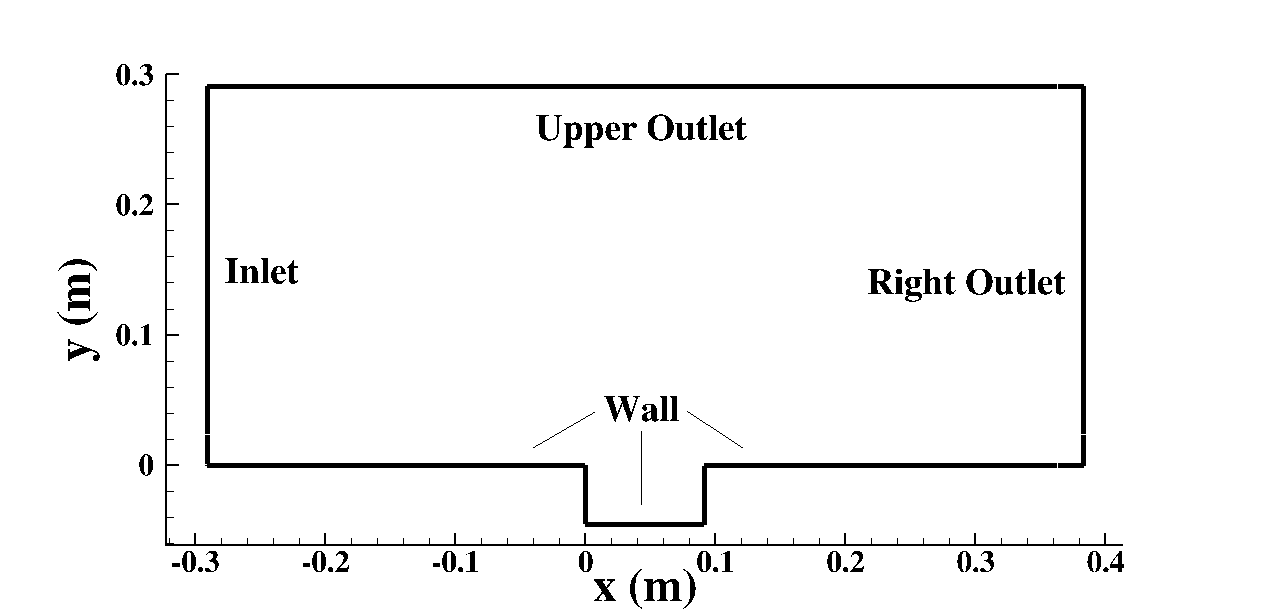
\includegraphics[width=0.9\linewidth]{Chapters/CavityAndCVRC/Images/cavity/geom.png}
	\fi
    \caption{\label{fig:cavityGeom} 2D transonic cavity flow domain.}
\end{figure}

The working gas is air, modeled as a calorically-perfect gas with the properties given in Table~\ref{tab:airProps}. Transport and thermodynamic properties are computed using the simplified analytical forms described in Section~\ref{subsec:gasModels}. The free-stream velocity is 208.7816 m/s in the +$x$-direction, the pressure is 25 Pa, and the temperature is 300 K. The working gas is air, modeled as a calorically-perfect gas (CPG) with the properties given in Table~\ref{tab:airProps}. The resulting Mach number of this flow regime is approximately 0.6, and the Reynolds number is approximately 6,500.

\begin{table}
	\centering
	\begin{tabular}{ lllll }
	\toprule
	MW (g/mol) & $c_p$ (kJ/kg-K) & $\mu$ (kg/m-s) & Pr & Sc   \\
	\midrule
	28.9604 & 1004.84 & 8.46e-7 & 0.72 & 0.62 \\
	\bottomrule
	\end{tabular}
	\caption{\label{tab:airProps}CPG properties of air for cavity flow case.}
\end{table}

The FOM is initialized with free stream conditions outside the cavity, and the inside of the cavity is initialized with free stream pressure and temperature, but zero velocity. The physical time step for the FOM simulation is $\dt = 1 \;\mu$s. Initial transients are allowed to dissipate and statistically-steady flow is established over 100 ms. After this point, the simulation is continued for 10 ms, during which the state is saved to disk at every physical time step, resulting in 10,001 snapshots (including $\stateVec\left(\timeVar = 100 \; \text{ms}\right)$). All ROM simulations are restarted from $\timeVar = 100 \; \text{ms}$. Several instantaneous flow field examples are shown in Figs.~\ref{fig:cavityPressExample}--\ref{fig:cavityVExampleZoom}. We draw particular attention to the oscillatory pressure field displayed in Fig.~\ref{fig:cavityPressExample}: this emission of pressure waves from the trailing edge of the cavity is the result of the shear layer (originating from leading edge) impinging on the trailing edge. The shear layer rollup (implied by the $y$-velocity field in Fig.~\ref{fig:cavityVExampleZoom}) due to the Helmholtz instability and the pressure perturbation that travels upstream results in several resonant tones. Pressure measurements at the aft wall over the 10 ms data collection period is shown in Fig.~\ref{fig:cavityFOMProbe}.

\begin{figure}
	\centering
	\ifdefined\DRAFT
		\includegraphics[width=0.9\linewidth]{example-image-a}
	\else
		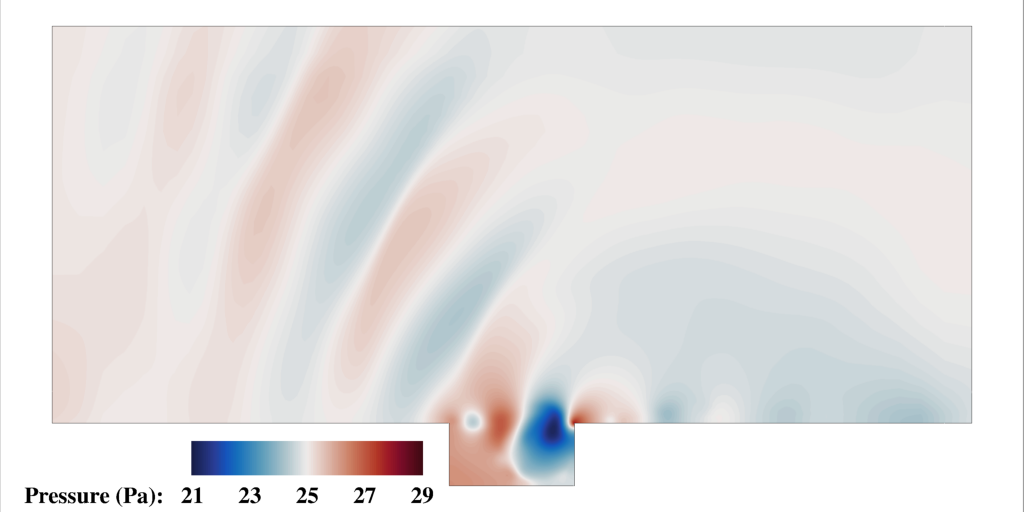
\includegraphics[width=0.9\linewidth,trim={0.5em 0.5em 0.5em 0.5em},clip]{Chapters/CavityAndCVRC/Images/cavity/pressure_example_full.png}
	\fi
	\caption{\label{fig:cavityPressExample}Pressure field at $\timeVar =$ 104 ms.}
\end{figure}

\begin{figure}
	\begin{minipage}{0.48\linewidth}
		\ifdefined\DRAFT
			\includegraphics[width=0.99\linewidth]{example-image-a}
		\else
			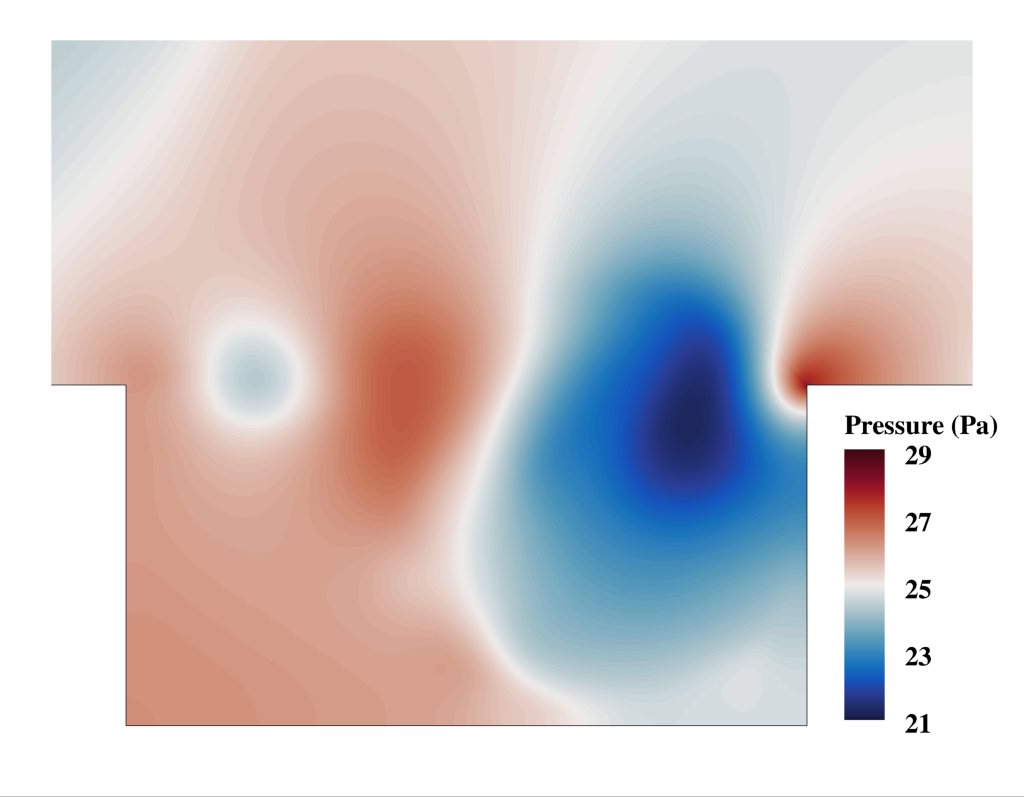
\includegraphics[width=0.99\linewidth,trim={0.5em 0.5em 0.5em 0.5em},clip]{Chapters/CavityAndCVRC/Images/cavity/pressure_example_zoom.png}
		\fi
		\caption{\label{fig:cavityPressExampleZoom}Pressure field at $\timeVar =$ 104 ms, zoomed cavity view.}
	\end{minipage} \hspace{0.5em}
	\begin{minipage}{0.48\linewidth}
		\ifdefined\DRAFT
			\includegraphics[width=0.99\linewidth]{example-image-a}
		\else
			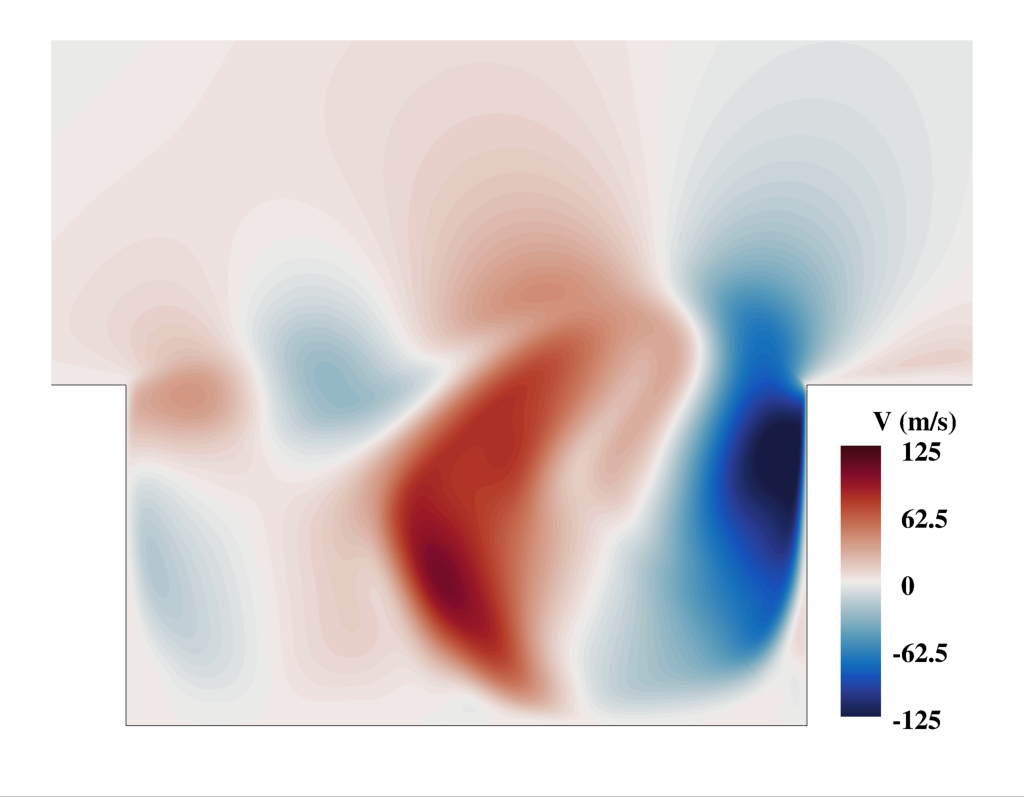
\includegraphics[width=0.99\linewidth,trim={0.5em 0.5em 0.5em 0.5em},clip]{Chapters/CavityAndCVRC/Images/cavity/y_vel_example_zoom.png}
		\fi
		\caption{\label{fig:cavityVExampleZoom}$y$-velocity field at $\timeVar =$ 104 ms, zoomed cavity view.}
	\end{minipage}
\end{figure}

For this flow regime and cavity geometry, the formula of Rossiter~\cite{Rossiter1964} (with $\alpha = 0.25$, $\kappa = 0.57$) predicts the first three acoustic modes to be $f = \{725.2, \; 1,692.1, \; 2,659.1\}$ Hz. As a rough confirmation of model suitability, 100 ms ($\timeVar \in [100, \; 200]$ ms) of pressure data is collected from the aft wall point monitor. The signal is filtered using a low-pass fifth-order Butterworth filter with a critical frequency of 20 kHz, and we compute the power spectral density by Welch's method with a window of 25 ms and 75\% window overlap. The resulting sound pressure level (SLP) is plotted in Fig.~\ref{fig:rossiterModeProof}, where the first three predicted Rossiter frequencies are marked in red. Although slightly overpredicting the first mode and underpredicting the third mode, we feel this is a reasonable match in comparing an empirical fit model and a two-dimensional numerical simulation.

\begin{figure}
	\begin{minipage}{0.48\linewidth}
		\ifdefined\DRAFT
			\includegraphics[width=0.99\linewidth]{example-image-a}
		\else
			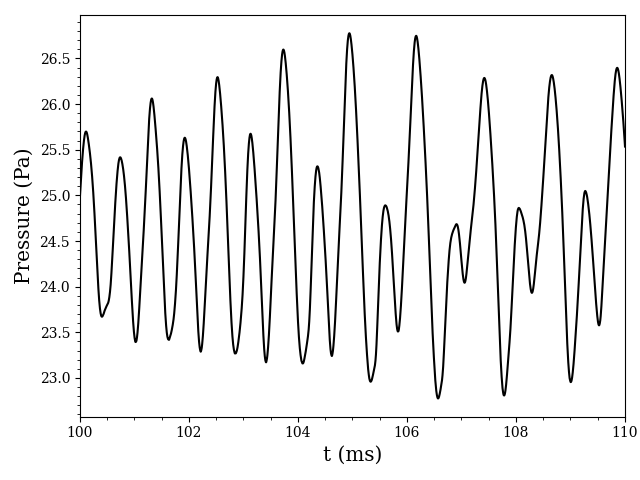
\includegraphics[width=0.99\linewidth,trim={0.5em 0.5em 0.5em 0.5em},clip]{Chapters/CavityAndCVRC/Images/cavity/pressure_probe_fom_10ms.png}
		\fi
		\caption{\label{fig:cavityFOMProbe}Pressure probe measurements from aft wall ($\timeVar \in [100, \; 110]$ ms).}
	\end{minipage} \hspace{0.5em}
	\begin{minipage}{0.48\linewidth}
		\ifdefined\DRAFT
			\includegraphics[width=0.99\linewidth]{example-image-a}
		\else
			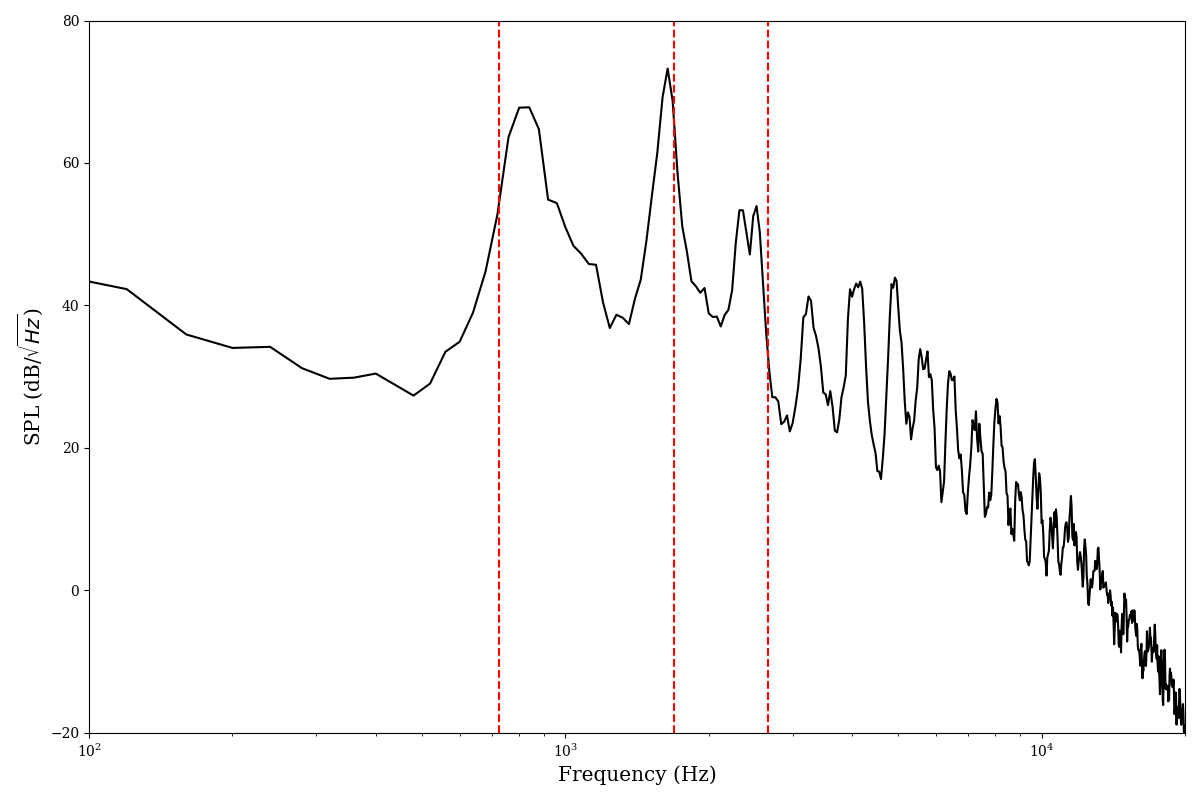
\includegraphics[width=0.99\linewidth,trim={0.5em 0.5em 0.5em 0.5em},clip]{Chapters/CavityAndCVRC/Images/cavity/psd_fom_100ms.png}
		\fi
		\caption{\label{fig:rossiterModeProof}Sound pressure level of aft wall pressure signal ($\timeVar \in [100, \; 200]$ ms). The first three Rossiter frequencies are marked in red.}
	\end{minipage}
\end{figure}

The POD trial bases are computed from the 10,001 snapshots of the conservative and primitive variables. The POD residual energy decay is displayed in Fig.~\ref{fig:cavityPODEnergy}. Achieving 1\%, 0.1\%, and 0.01\% of the conservative state POD residual energy requires 20, 73, and 155 modes respectively. For the primitive state, this increases to 26, 92, and 180 modes respectively. Although this is a fairly simple problem without any reaction phenomena, this slow POD residual energy decay exhibits how traveling waves and large fluctuations in the unsteady flow field can require a large number of trial bases to approximate accurately. Indeed, the primitive and conservative variable projection error plots in Fig.~\ref{fig:cavityProjErr} indicate that over 125 modes are required to decrease the projection error of the  and velocity and momentum magnitudes below 0.1\% relative error.

\begin{figure}
	\centering
	\ifdefined\DRAFT
		\includegraphics[width=0.8\linewidth]{example-image-a}
	\else
		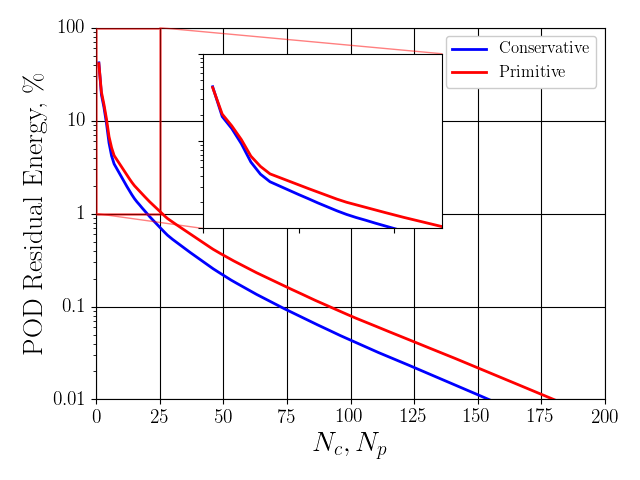
\includegraphics[width=0.8\linewidth]{Chapters/CavityAndCVRC/Images/cavity/cavity_pod_energy_10ms.png}
	\fi
	\caption{\label{fig:cavityPODEnergy}POD residual energy decay for 2D cavity flow conservative and primitive state datasets.}
\end{figure}

\begin{figure}
	\begin{minipage}{0.48\linewidth}
		\ifdefined\DRAFT
			\includegraphics[width=0.99\linewidth]{example-image-a}
		\else
			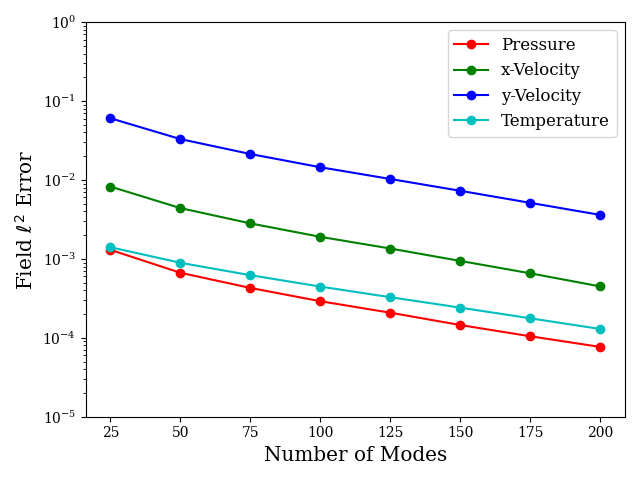
\includegraphics[width=0.99\linewidth,trim={0.5em 0.5em 0.5em 0.5em},clip]{Chapters/CavityAndCVRC/Images/cavity/projection_error_primitive.png}
		\fi
		\subcaption{Primitive variables.}
	\end{minipage} \hspace{0.5em}
	\begin{minipage}{0.48\linewidth}
		\ifdefined\DRAFT
			\includegraphics[width=0.99\linewidth]{example-image-a}
		\else
			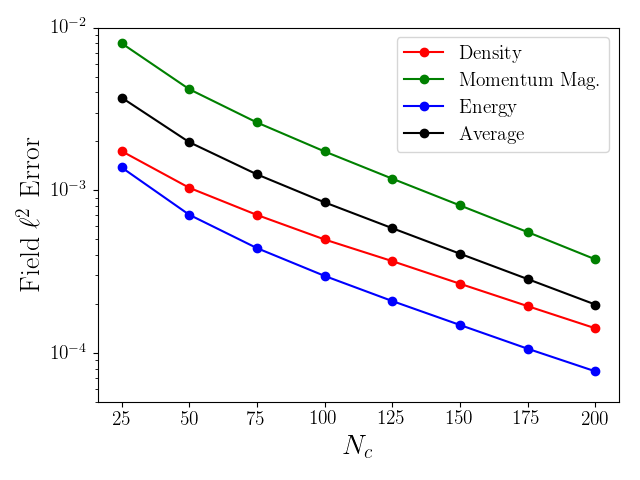
\includegraphics[width=0.99\linewidth,trim={0.5em 0.5em 0.5em 0.5em},clip]{Chapters/CavityAndCVRC/Images/cavity/projection_error_conservative.png}
		\fi
		\subcaption{Conservative variables.}
	\end{minipage}
	\caption{\label{fig:cavityProjErr}Time-average POD projection error.}
\end{figure}

\subsection{Unsampled PROMs}

\begin{figure}
	\begin{minipage}{0.49\linewidth}
		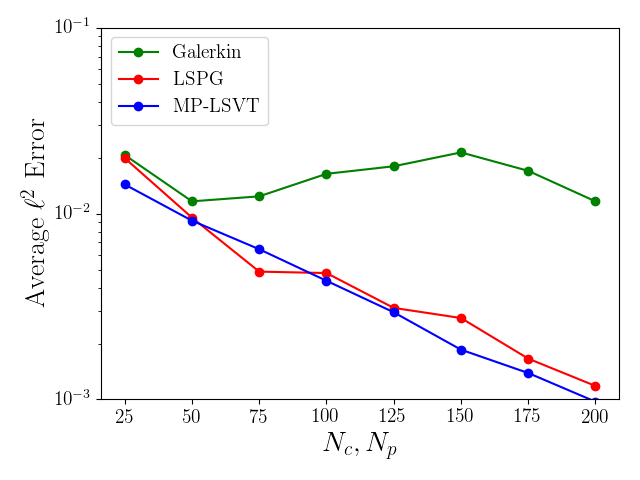
\includegraphics[width=0.99\linewidth]{Chapters/CavityAndCVRC/Images/cavity/unsampled/unsampled_dt1e-6_Average_errorRaw.png}
		\subcaption{$\dt = \dtFOM$}
	\end{minipage}
	\begin{minipage}{0.49\linewidth}
		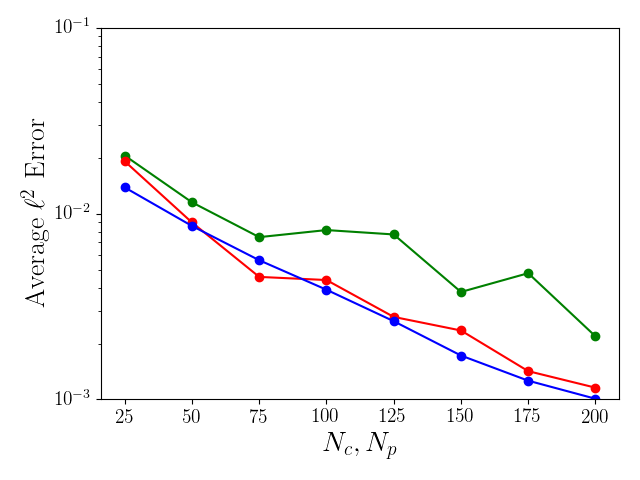
\includegraphics[width=0.99\linewidth]{Chapters/CavityAndCVRC/Images/cavity/unsampled/unsampled_dt2p5e-6_Average_errorRaw.png}
		\subcaption{$\dt = 2.5 \times \dtFOM$}
	\end{minipage}

	\begin{minipage}{0.49\linewidth}
		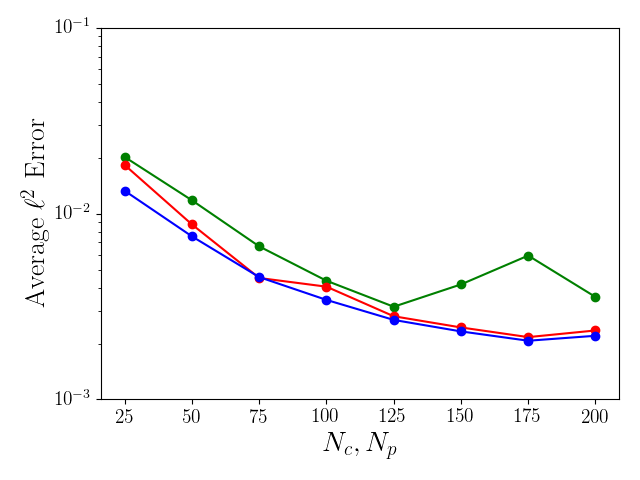
\includegraphics[width=0.99\linewidth]{Chapters/CavityAndCVRC/Images/cavity/unsampled/unsampled_dt5e-6_Average_errorRaw.png}
		\subcaption{$\dt = 5 \times \dtFOM$}
	\end{minipage}
	\begin{minipage}{0.49\linewidth}
		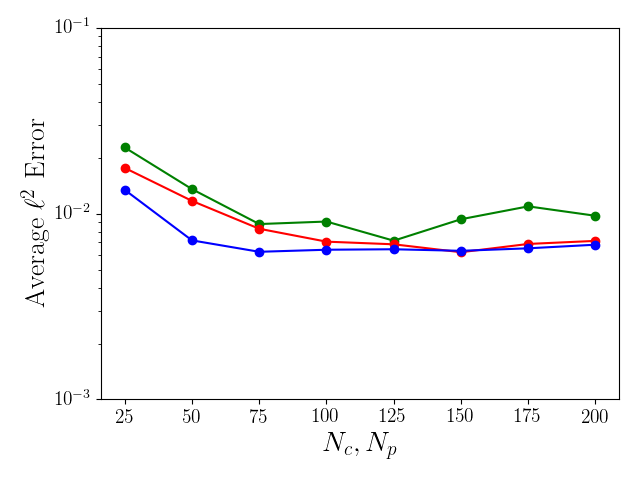
\includegraphics[width=0.99\linewidth]{Chapters/CavityAndCVRC/Images/cavity/unsampled/unsampled_dt1e-5_Average_errorRaw.png}
		\subcaption{$\dt = 10 \times \dtFOM$}
	\end{minipage}
	\caption{\label{fig:cavityUnsampledROMErrVsModes}2D cavity unsampled ROM time-average error, various $\dt$}
\end{figure}